\documentclass[11pt]{article}

\usepackage{fullpage}
\usepackage{rotating}   
\usepackage{amsmath}
\usepackage{amssymb}
\usepackage{amsthm}
\usepackage{fancyhdr}
\usepackage{algorithm}
\usepackage{algorithmic}
\usepackage{bm}
\usepackage{listings}
\usepackage{graphicx}
\usepackage{caption2}
\usepackage{subfigure}
\usepackage{float}
\usepackage{extpfeil}
\usepackage{color}
\usepackage[usenames,dvipsnames]{xcolor}


\newtheorem{theorem}{Theorem}[section]
\newtheorem{lemma}[theorem]{Lemma}
\newtheorem{corollary}[theorem]{Corollary}
\newtheorem{proposition}[theorem]{Proposition}
\newtheorem{definition}[theorem]{Definition}
\newtheorem{conjecture}[theorem]{Conjecture}
\newtheorem{remark}[subsection]{Remark}

%%
\newcommand\numberthis{\addtocounter{equation}{1}\tag{\theequation}}

%% define new symbols
\def\bx{\bm{x}}
\def\bb{\bm{b}}
\def\ba{\bm{a}}
\def\bc{\bm{c}}
\def\bf{\bm{f}}
\def\by{\bm{y}}
\def\bu{\bm{u}}
\def\bv{\bm{v}}
\def\BW{\bm{W}}
\def\BA{\bm{A}}
\def\bz{\bm{z}}
\def\BZ{\bm{Z}}
\def\BH{\bm{H}}
\def\BL{\bm{L}}
\def\BU{\bm{U}}
\def\BV{\bm{V}}
\def\BB{\bm{B}}
\def\BC{\bm{C}}
\def\BD{\bm{D}}
\def\BE{\bm{E}}
\def\BW{\bm{W}}
\def\BQ{\bm{Q}}
\def\BG{\bm{G}}
\def\BA{\bm{A}}
\def\BX{\bm{X}}
\def\BY{\bm{Y}}
\def\BQ{\bm{Q}}
\def\BI{\bm{I}}
\def\BR{\bm{R}}

%% define new brackets
\def\la{\left\langle}
\def\ra{\right\rangle}
\def\ln{\left\|}
\def\rn{\right\|}
\def\lb{\left(}
\def\rb{\right)}
\def\lsb{\left[}
\def\rsb{\right]}
\def\lcb{\left\{}
\def\rcb{\right\}}

%%
\DeclareMathOperator*{\argmin}{arg\,min}
\DeclareMathOperator*{\argmax}{arg\,max}

%%
\title{Homework IV}
\author{Name: Shao Yanjun, Number: 19307110036}


\begin{document}
\maketitle

%------------------------------------
\begin{abstract}
This is Daniel's homework of  "Numerical Algorithms with Case Studies II".
\end{abstract}
%-------------------------------------
%=====================
\section{Problems}
\paragraph{Q1}
It is clear that the difference quotient $f[x_1,x_2,\cdots,x_k]$ is the leading coefficienct of the $k-1^{th}$ interpolation polynomial $P(x)$ at the points $(x_1,x_2,\cdots,x_k)$. That is to say, the difference function $g(x)=P(x)-f(x)$ has at least k different zero points. Applying Rolle's Theorem, we discover that,
\begin{align}
g^{(k-1)}(\xi)=(k-1)!\cdot f[x_1,x_2,\cdots,x_k]&-f^{(k-1)}(\xi)=0
,\quad\exists \xi\in(min\{x_i\},max\{x_i\})\\ \therefore
f[x_1,x_2,\cdots,x_k]&=\frac{f^{(k-1)}(\xi)}{(k-1)!}
\end{align}
\qquad When $(x_1,x_2,\cdots,x_k)\rightarrow(x_*,x_*,\cdots,x_*)$, we have $max\{x_i\}\rightarrow x_*$ and $min\{x_i\}\rightarrow x_*$. So we have $\xi\rightarrow x_*$.
\begin{align}
	\therefore \lim_{(x_1,x_2,\cdots,x_k)\rightarrow(x_*,x_*,\cdots,x_*)} f[x_1,x_2,\cdots,x_k]&=\frac{f^{(k-1)}(x_*)}{(k-1)!}
\end{align}
\paragraph{Q2}
We first define the difference of a function.
\begin{definition}
	The $1^{st}$ difference is denoted as $\Delta f(x_i)=f(x_{i+1})-f(x_i)$. 
	The $2^{nd}$ difference is denoted as $\Delta^2 f(x_i)=\Delta f(x_{i+1})-\Delta f(x_i)$. And the $k^{th}$ difference is denoted as $\Delta^{(k)}f(x_i)=\Delta^{(k-1)}f(x_{i+1})-
	\Delta^{(k-1)}f(x_i)$ subsequently.
\end{definition}
\, After calculating,
\begin{align}
	\Delta^2 f(x_i)=\Delta f(x_{i+1})-\Delta f(x_i)=f(x_{i+2})-2f(x_{i+1})+f(x_i)
\end{align} 
\qquad We could induce for every $k\in \mathbb{N}$
\begin{align}
	\Delta^{(k)}f(x_i)&=\Delta^{(k-1)}f(x_{i+1})-
	\Delta^{(k-1)}f(x_i)\\&=f(x_{i+k})-(\binom{k-1}{1}+1)f(x_{i+k-1})+\cdots+(-1)^k f(x_i)\\
	&=f(x_{i+k})-\binom{k}{1}f(x_{i+k-1})+\binom{k}{2}f(x_{i+k-2})\cdots+(-1)^k f(x_i)
\end{align}
\qquad And we can calculate the coefficients of the polynomial with the following table.\\

\begin{center}
\begin{tabular}{ccccccc}
&$x_1$ &$f(x_1)$ &$\frac{\Delta f(x_1)}{h}$ &$\cdots$ 
&$\frac{\Delta ^{(n-1)}f(x_1)}{(n-1)!h^{(n-1)}}$ &$\frac{\Delta ^{(n)}f(x_1)}{n!h^n}$\\

&$x_1+h$ &$f(x_1+h)$ &$\frac{\Delta f(x_2)}{h}$ &$\cdots$ 
&$\frac{\Delta ^{(n-1)}f(x_2)}{(n-1)!h^{(n-1)}}$&\\

&$\vdots$ &$\vdots$ &$\vdots$ &\begin{turn}{90}$\ddots$\end{turn}&&\\
&$x_1+(n-1)h$ &$f(x_1+(n-1)h)$
\end{tabular}
\end{center}
\qquad We take out the first row of the table to be the coefficients of our polynomial, that is, $c_0=f(x_1)$, $c_1=\frac{\Delta f(x_1)}{h}$, $\cdots$, $c_n=\frac{\Delta ^{(n)}f(x_1)}{n!h^n}$. The polynomial can be simplified as follows.
\begin{align}
	P(x)=c_0+c_1(x-x_1)+\cdots+c_n(x-x_1)(x-x_2)\cdots(x-x_{n-1})
\end{align}
\paragraph{Q3}
Apply my algorithm and make the plottings and error analysis (relative),
\begin{figure}[H]
	\centering
	\subfigure[interpolation of sin(x)]{
		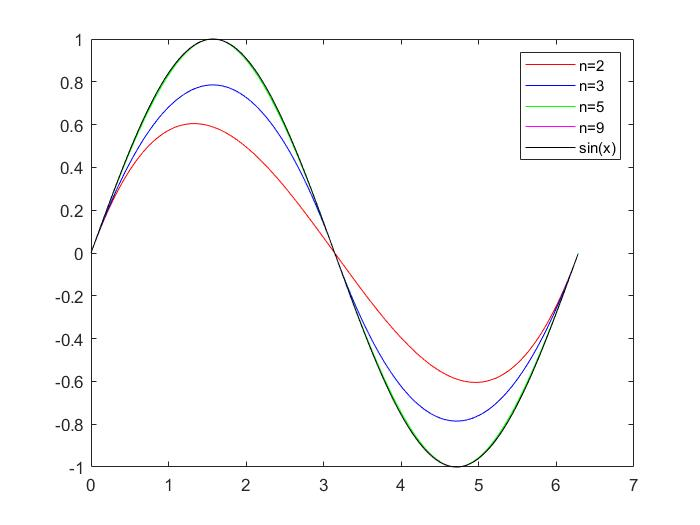
\includegraphics[width=0.4\linewidth]{H4Q3_1.jpg}
	}
	\subfigure[error analysis]{
		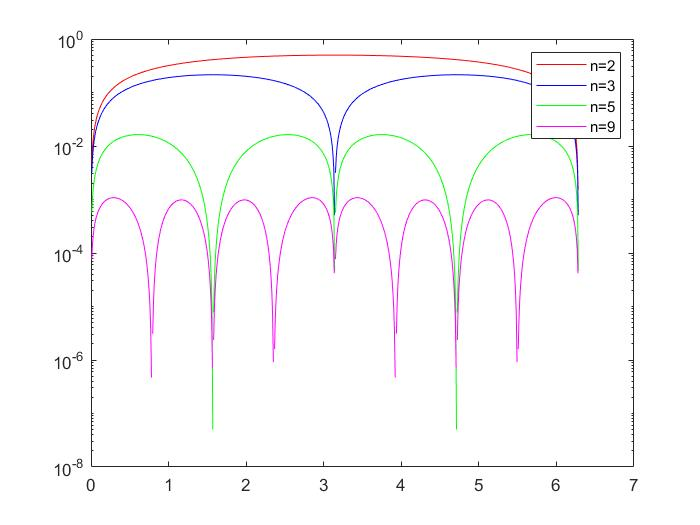
\includegraphics[width=0.4\linewidth]{H4Q3_2.jpg}
	}
\end{figure}
\paragraph{Q4}
We prefer Newton's interpolation over Lagrange's interpolation, because it's easier to implement.
\begin{figure}[H]
	\centering
	\subfigure[interpolation of my function]{
		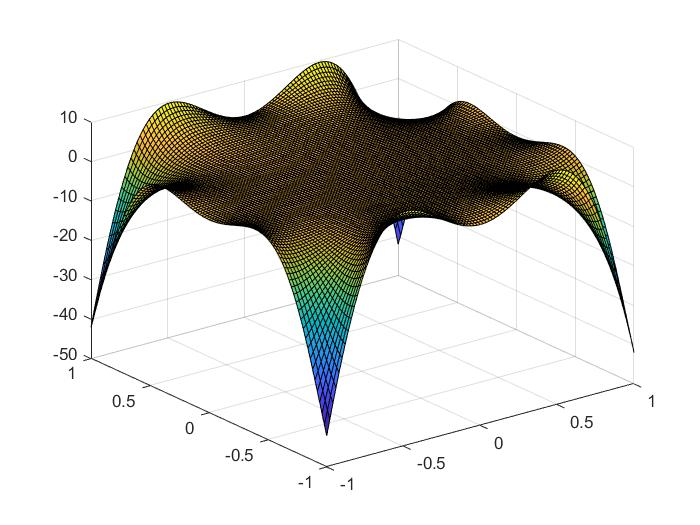
\includegraphics[width=0.6\linewidth]{H4Q4.jpg}
	}
\end{figure}

%-------------------------------------
%=====================
\end{document}
